\documentclass{beamer}

\usepackage[utf8]{inputenc}
\usepackage{graphicx}


\title{Digitale Transformation in Wirtschaft und Gesellschaft}
\author{Milestone 07.05.20}
\institute{University of Bamberg/ University Konstanz}
\date{2020}



\begin{document}

\frame{\titlepage}

\begin{frame}
\frametitle{Our Team}

\begin{itemize}
	\item 4 Bachelor Students (Winf \& IS) 
	\item 1 Master Student  (Data Science)
\end{itemize}



%Interdisziplinäres Team mit einem verschiedenen Level an Erfahrungen. Für einige ist dies das erste Seminar, andere wiederum haben schon etwas mehr Erfahrung und andere haben auch schon Erfahrungen im Themengebiet gesammelt.

\end{frame}


\begin{frame}
\frametitle{Introduction into the topic}
 Bill Gates, together with his foundation has occupied a leading role in the global fight against COVID-19. He received a lot of media coverage on the traditional media and social media in the past weeks, but not all coverage is positive. An increasing amount of content that is produced around the name of Bill Gates accuses him of things like microchipping humanity to control them or being responsible for the outbreak of COVID-19.
\end{frame}	

\begin{frame}
\frametitle{Introduction into the topic}
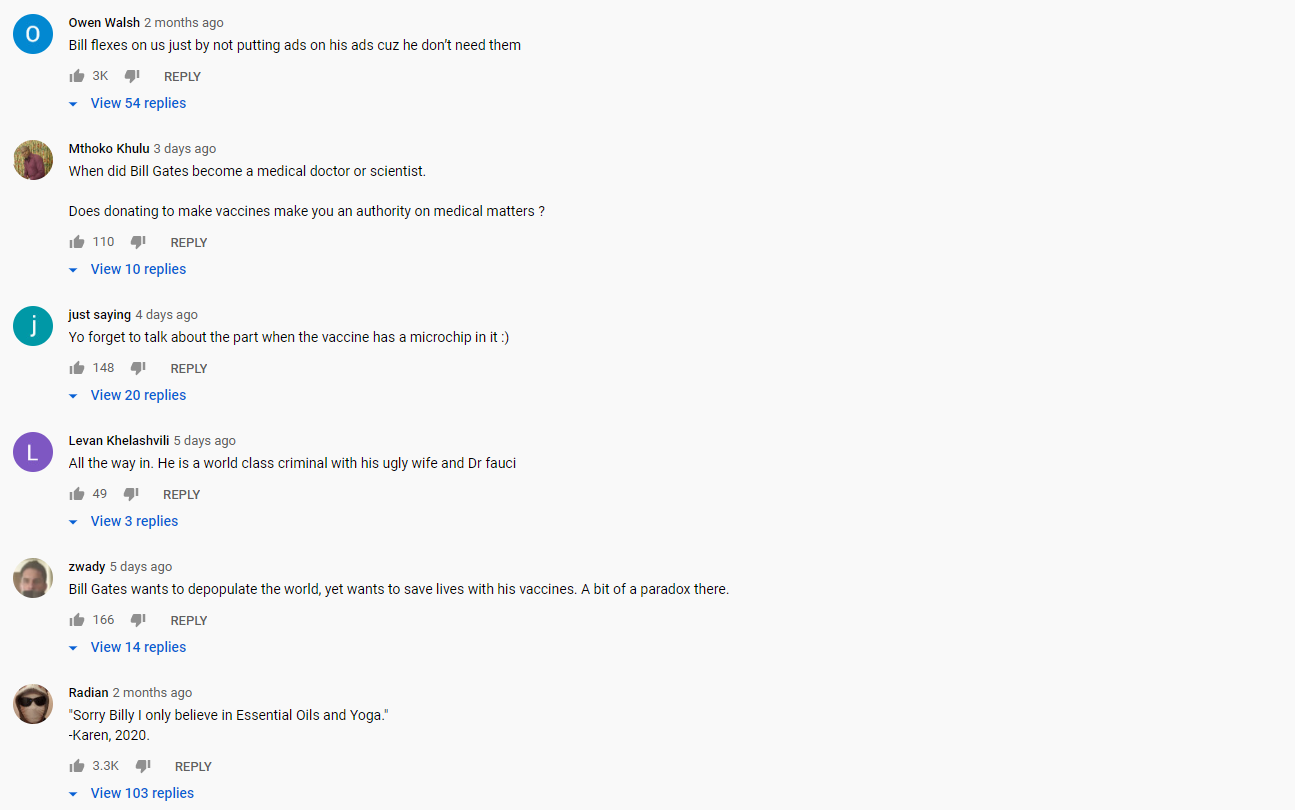
\includegraphics[height=0.7\textheight]{BillGatesvaccines}
Source: youtube.com/watch?v=hh6xTguRn9o
\end{frame}	


\begin{frame}
\frametitle{Introduction into the topic}
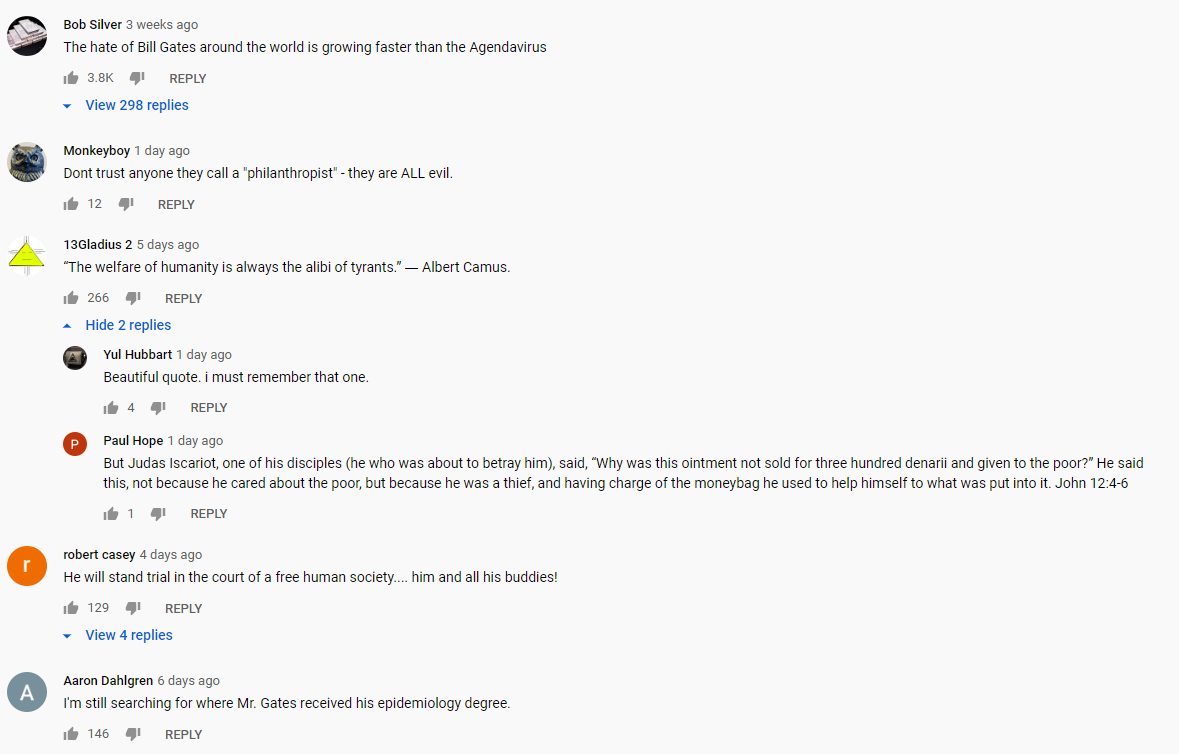
\includegraphics[height=0.7\textheight]{BillGatesResponds}
Source: https://www.youtube.com/watch?v=nFUdX\_0PpT0
\end{frame}	
\begin{frame}
\frametitle{Research Question}
\begin{center}
Is their a correlation between the frequency of which videos are recommended and the political  view of those videos? 
\end{center}

\end{frame}	


\begin{frame}
\frametitle{Data Gathering}

\begin{itemize}
	\item Gathering of the natural language through the provided subtitles by YouTube
	\item Interfaces: YouTube API and YouTube -dl
	\item Tools: Python 
	
\end{itemize}
\end{frame}	

\end{document}